\chapter{Pembakaran: Bahan Bakar, Produk, dan Gas Rumah Kaca}\label{ch:g8:combustion-and-fuels}

Sebuah keluarga tidur di apartemen yang cerobong pemanas airnya
tersumbat. Nyala gasnya, yang kekurangan \omterm{def:g4:air-a-mixture-of-gases:air}{udara}, menyala buruk, dan
sejenis gas yang tidak terlihat dan tidak berbau perlahan memenuhi
ruangan. Pukul dua pagi, sebuah kotak kecil di dinding mulai menjerit:
alarm karbon monoksida. Semua orang keluar tepat pada waktunya. \omterm{def:g4:what-a-fire-needs:fuel}{Bahan
bakar} yang sama, bila menyala dengan baik, hanya menghasilkan karbon
dioksida dan air --- dan karbon dioksida itu punya kisahnya sendiri,
yang tertulis di \omterm{def:g4:air-a-mixture-of-gases:air}{udara} seluruh planet.

\begin{recall}
\omterm{def:g4:what-a-fire-needs:burning}{Pembakaran} memerlukan \omterm{def:g4:what-a-fire-needs:fuel}{bahan bakar}, oksigen, dan panas, dan menghasilkan
zat-zat baru (\cref{ch:g4:what-a-fire-needs}). \omterm{def:g4:air-a-mixture-of-gases:air}{Udara} terdiri atas
sekitar seperlima oksigen (\cref{ch:g4:air-a-mixture-of-gases}).
Sebuah \omterm{def:g8:balanced-equations:equation}{persamaan setara} jika setiap jenis \omterm{def:g7:atoms-and-molecules:atom}{atom} muncul sama banyak di
kedua ruas (\cref{ch:g8:balanced-equations}).
\end{recall}

\section{Pembakaran karbon dan metana}

\begin{example}[Dua pembakaran]\label{ex:g8:combustion-and-fuels:two}
Karbon (arang, batu bara) \omterm{def:g4:what-a-fire-needs:burning}{terbakar} menghasilkan karbon dioksida:
\[
  \ce{C(s) + O2(g) -> CO2(g)}.
\]
Metana, bagian utama gas alam, \omterm{def:g4:what-a-fire-needs:burning}{terbakar} menghasilkan karbon dioksida dan
air:
\[
  \ce{CH4(g) + 2O2(g) -> CO2(g) + 2H2O(l)}.
\]
Dalam kedua kasus, air kapur menjadi keruh oleh gas yang terbentuk;
dengan metana, gelas dingin juga berembun.
\end{example}

\begin{method}[Menuliskan pembakaran bahan bakar yang terdiri atas karbon dan hidrogen]\label{met:g8:combustion-and-fuels:write}
Untuk \omterm{def:g4:what-a-fire-needs:fuel}{bahan bakar} yang \omterm{def:g7:atoms-and-molecules:molecule}{molekulnya} hanya mengandung karbon dan hidrogen:
\begin{enumerate}
  \item produknya adalah karbon dioksida dan air;
  \item setarakan karbon dengan \ce{CO2}, lalu hidrogen dengan \ce{H2O};
  \item hitung \omterm{def:g7:atoms-and-molecules:atom}{atom} oksigen di kanan dan setarakan dengan \ce{O2};
        gandakan semuanya jika muncul bilangan setengah.
\end{enumerate}
Untuk butana: \ce{2C4H10 + 13O2 -> 8CO2 + 10H2O}.
\end{method}

\section{Pembakaran sempurna dan tidak sempurna}

\begin{definition}[Pembakaran sempurna dan tidak sempurna]\label{def:g8:combustion-and-fuels:complete}
Sebuah \emph{pembakaran sempurna}\index{pembakaran sempurna} berlangsung
dengan oksigen yang cukup: semua karbon dalam \omterm{def:g4:what-a-fire-needs:fuel}{bahan bakar} menjadi karbon
dioksida. Sebuah
\emph{pembakaran tidak sempurna}\index{pembakaran tidak sempurna}
berlangsung dengan oksigen yang terlalu sedikit: sebagian karbonnya
menjadi karbon monoksida, \ce{CO}, atau jelaga, yaitu karbon, \ce{C}.
\end{definition}

\begin{example}[Metana yang kekurangan oksigen]\label{ex:g8:combustion-and-fuels:incomplete}
Dengan \omterm{def:g4:air-a-mixture-of-gases:air}{udara} yang terlalu sedikit, metana dapat \omterm{def:g4:what-a-fire-needs:burning}{terbakar} menjadi karbon
monoksida atau jelaga:
\[
  \ce{2CH4 + 3O2 -> 2CO + 4H2O}, \qquad \ce{CH4 + O2 -> C + 2H2O}.
\]
\end{example}

\begin{proposition}[Membaca nyala api]\label{prop:g8:combustion-and-fuels:flame}
Pembakar Bunsen dengan lubang \omterm{def:g4:air-a-mixture-of-gases:air}{udara} terbuka \omterm{def:g2:mixing-and-dissolving:mix}{mencampurkan} \omterm{def:g4:air-a-mixture-of-gases:air}{udara} ke dalam
gas sebelum gas itu \omterm{def:g4:what-a-fire-needs:burning}{terbakar}: nyalanya biru dan hampir tidak terlihat,
\omterm{def:g4:what-a-fire-needs:burning}{pembakarannya} sempurna. Dengan lubang \omterm{def:g4:air-a-mixture-of-gases:air}{udara} tertutup, gas itu hanya
mendapat sedikit oksigen: nyalanya kuning, berasap, dan menghitamkan
benda dingin yang dipegang di dalamnya dengan jelaga --- \omterm{def:g4:what-a-fire-needs:burning}{pembakarannya}
tidak sempurna.
\end{proposition}

\begin{omfigure}
\begin{tikzpicture}[font=\small, scale=1.3]
  \pic[transform shape] at (0,0) {bunsen=open};
  \node[anchor=north, align=center] at (0,-0.1) {lubang udara terbuka:\\ nyala biru, sempurna};
  \pic[transform shape] at (4,0) {bunsen=closed};
  \node[anchor=north, align=center] at (4,-0.1) {lubang udara tertutup:\\ nyala kuning, tidak sempurna};
  \draw[<-, omProp, thick] (0.08,0.6) -- (1.4,0.9) node[right, text=black] {lubang udara};
  \draw[<-, omProp, thick] (-0.4,0.3) -- (-1.3,0.6) node[left, text=black] {gas};
  \draw[<-, omProp, thick] (4.15,3.3) -- (5.0,3.5) node[right, text=black, align=left]
    {jelaga, karbon\\ monoksida};
\end{tikzpicture}

{\small Pembakar Bunsen. \omterm{def:g4:air-a-mixture-of-gases:air}{Udara} yang masuk dari bawah menghasilkan nyala
biru dan \omterm{def:g8:combustion-and-fuels:complete}{pembakaran sempurna}; tanpa \omterm{def:g4:air-a-mixture-of-gases:air}{udara} itu nyalanya kuning dan
berasap.}
\end{omfigure}

\begin{omfigure}
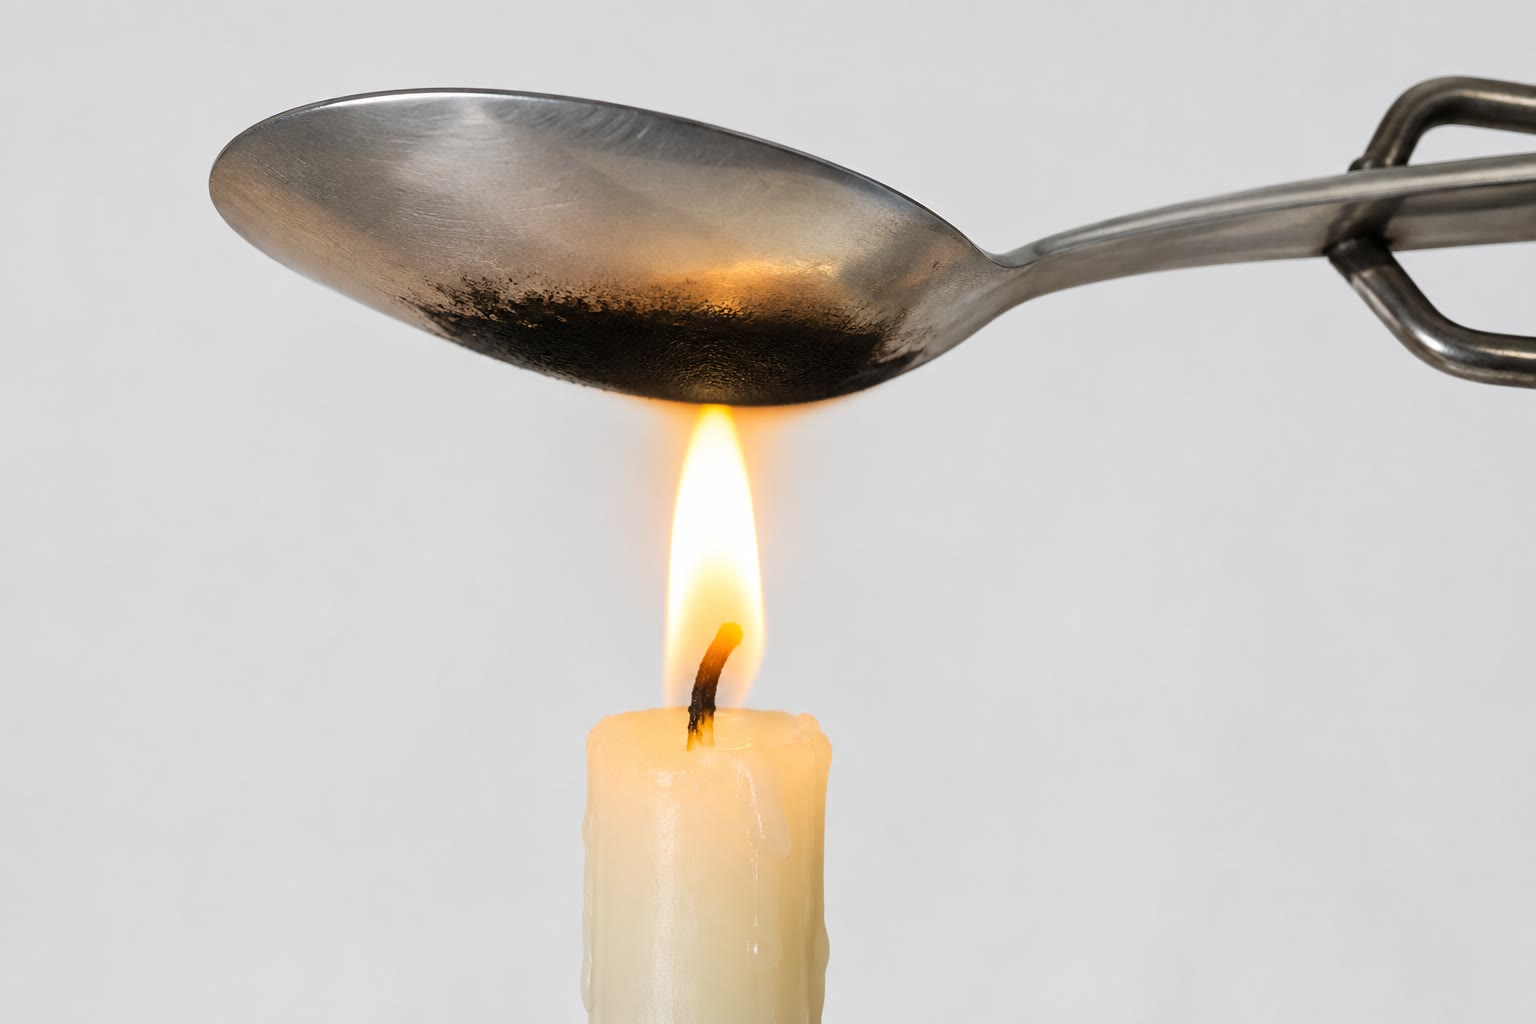
\includegraphics[width=0.45\linewidth]{images/book1/ai/g8-soot-spoon.jpg}

{\small Sendok dingin yang dipegang di dalam nyala lilin yang kuning
menjadi hitam oleh jelaga: \omterm{def:g4:what-a-fire-needs:burning}{pembakarannya} tidak sempurna.}
\end{omfigure}

\section{Karbon monoksida, bahaya yang senyap}

\begin{proposition}[Mengapa karbon monoksida mematikan]\label{prop:g8:combustion-and-fuels:co}
Karbon monoksida tidak berwarna, tidak berbau, dan tidak berasa. Jika
terhirup, gas itu menggantikan tempat oksigen di dalam darah (buku
biologi menjelaskan caranya), menyebabkan sakit kepala, kantuk, dan di
ruangan tertutup pingsan dan kematian. Gas ini dihasilkan oleh \omterm{def:g4:what-a-fire-needs:fuel}{bahan
bakar} apa pun yang \omterm{def:g4:what-a-fire-needs:burning}{terbakar} dengan \omterm{def:g4:air-a-mixture-of-gases:air}{udara} yang kurang: pemanas air gas
yang kurang terawat atau cerobongnya tersumbat, kompor di dalam tenda
tertutup, pemanggang atau genset yang dipakai di dalam ruangan.
\end{proposition}

\begin{safety}{\ghs[0.8cm]{GHS02}\ghs[0.8cm]{GHS04}\ghs[0.8cm]{GHS06}\ghs[0.8cm]{GHS08}}
% ledger: ghs:CO
Karbon monoksida: gas yang sangat mudah menyala (GHS02), disediakan di
bawah tekanan (GHS04); beracun jika terhirup (GHS06); merusak organ
melalui paparan berulang dan dapat membahayakan janin (GHS08).
\end{safety}

\begin{remark}[Mencegah keracunan]\label{rem:g8:combustion-and-fuels:prevent}
Peralatan gas dirawat secara berkala oleh tenaga ahli, cerobong dan
lubang ventilasi tidak pernah ditutup, pemanggang dan genset hanya
dipakai di luar ruangan, dan alarm karbon monoksida dipasang di dekat
setiap pembakar.
\end{remark}

\begin{omfigure}
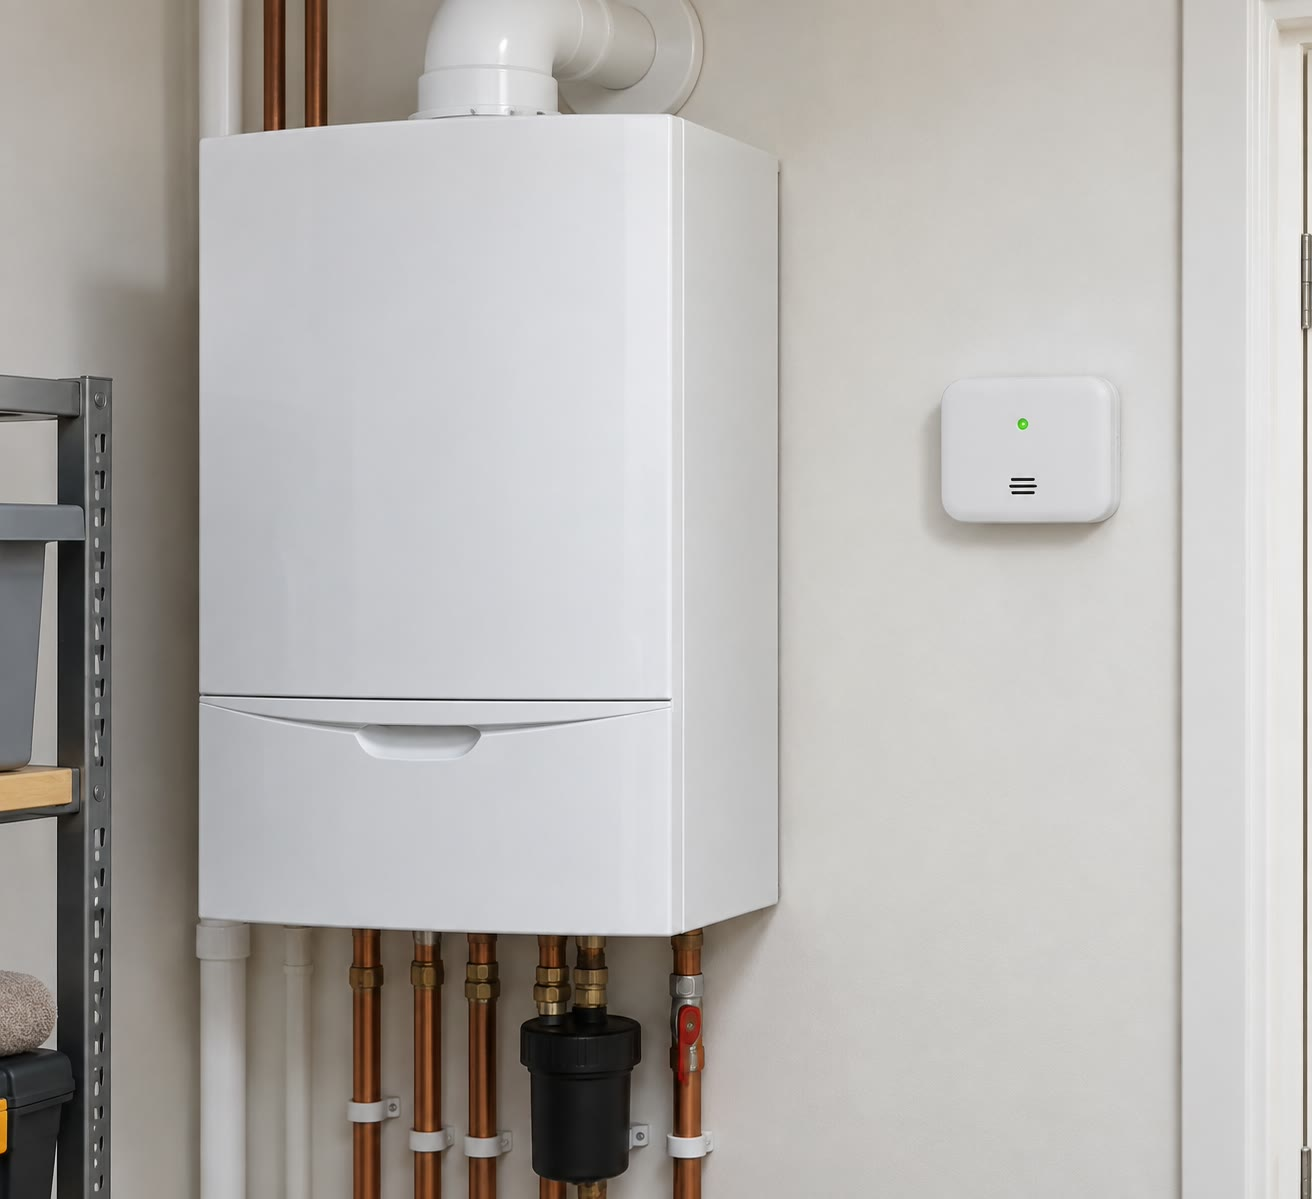
\includegraphics[width=0.45\linewidth]{images/book1/ai/g8-boiler-alarm.jpg}

{\small Pemanas air gas dan, di sampingnya, alarm karbon monoksida.}
\end{omfigure}

\section{Karbon dioksida dan efek rumah kaca}

\begin{definition}[Gas rumah kaca]\label{def:g8:combustion-and-fuels:greenhouse}
Yang disebut \emph{gas rumah kaca}\index{gas rumah kaca} adalah gas di
\omterm{def:g4:air-a-mixture-of-gases:air}{udara} yang meneruskan cahaya matahari tetapi menahan sebagian panas yang
dipancarkan kembali oleh permukaan Bumi ke arah antariksa, sehingga
menghangatkan atmosfer bagian bawah. Uap air, karbon dioksida, dan
metana adalah gas rumah kaca; nitrogen dan oksigen bukan. (Cara
terjadinya dijelaskan di buku fisika.)
\end{definition}

\begin{proposition}[Karbon dioksida di udara terus naik]\label{prop:g8:combustion-and-fuels:rising}
% ledger: co2:mlo-1959, co2:mlo-2025 (rise 111.4 ppm, +35 %)
Jumlah karbon dioksida di \omterm{def:g4:air-a-mixture-of-gases:air}{udara} telah diukur tanpa terputus sejak 1959
di sebuah observatorium di puncak gunung di tengah Samudra Pasifik.
Jumlahnya 316 bagian per juta (ppm) \omterm{def:g4:air-a-mixture-of-gases:air}{udara} pada tahun 1959 dan 427 ppm
pada tahun 2025: naik sekitar \qty{35}{\percent} dalam rentang satu
umur manusia, sebagian besar akibat \omterm{def:g4:what-a-fire-needs:burning}{pembakaran} batu bara, minyak bumi,
dan gas alam. Karbon dioksida tambahan itu memperkuat efek rumah kaca
dan menghangatkan iklim.
\end{proposition}

\begin{omfigure}
\begin{tikzpicture}
\begin{axis}[width=0.85\linewidth, height=6cm, xmin=1955, xmax=2030,
    ymin=300, ymax=440, xlabel={tahun}, ylabel={karbon dioksida (ppm)},
    axis lines*=left, ymajorgrids, grid style={gray!20},
    tick label style={font=\small, /pgf/number format/1000 sep={}},
    label style={font=\small}]
\addplot[omDef, thick, mark=*, mark size=0.8pt]
  table[x=year, y=ppm] {figdata/out/grade-8-co2-record.dat};
\node[anchor=west, font=\small] at (axis cs:1962,306) {316 ppm pada 1959};
\node[anchor=east, font=\small] at (axis cs:2023,428) {427 ppm pada 2025};
\end{axis}
\end{tikzpicture}

{\small Rata-rata tahunan karbon dioksida di \omterm{def:g4:air-a-mixture-of-gases:air}{udara}, diukur sejak 1959
(data NOAA Global Monitoring Laboratory; sebelum 1974, Scripps
Institution of Oceanography).}
\end{omfigure}

\section{Bahan bakar fosil dan terbarukan}

\begin{definition}[Bahan bakar fosil dan terbarukan]\label{def:g8:combustion-and-fuels:fossil}
Sebuah \emph{bahan bakar fosil}\index{bahan bakar fosil} --- batu bara,
minyak bumi, gas alam --- terbentuk di bawah tanah selama jutaan tahun
dari sisa-sisa tumbuhan dan makhluk laut purba. Sebuah
\emph{bahan bakar terbarukan}\index{bahan bakar terbarukan} dibuat dari
tumbuhan yang tumbuh sekarang, atau dari sampah: kayu, biogas dari
kotoran ternak dan sisa makanan, etanol yang dibuat dari bit gula atau
tebu.
\end{definition}

\begin{proposition}[Dari mana karbonnya berasal]\label{prop:g8:combustion-and-fuels:cycle}
Tumbuhan mengambil karbon dioksida dari \omterm{def:g4:air-a-mixture-of-gases:air}{udara} untuk tumbuh. Membakar
\omterm{def:g8:combustion-and-fuels:fossil}{bahan bakar terbarukan} mengembalikan karbon dioksida yang diambil
tumbuhannya dari \omterm{def:g4:air-a-mixture-of-gases:air}{udara} beberapa tahun sebelumnya. Membakar \omterm{def:g8:combustion-and-fuels:fossil}{bahan bakar
fosil} melepaskan karbon yang tersimpan di bawah tanah selama jutaan
tahun: karbon dioksida di \omterm{def:g4:air-a-mixture-of-gases:air}{udara} bertambah.
\end{proposition}

\begin{omfigure}
\begin{tikzpicture}[font=\small,
    box/.style={draw=omDef, fill=omDef!6, rounded corners=2pt, align=center,
      minimum height=0.9cm, text width=2.6cm}]
  \node[box] (air) at (0,3) {karbon dioksida\\ di udara};
  \node[box] (plants) at (5.6,3) {tumbuhan\\ tumbuh\\ (menyerap \ce{CO2})};
  \node[box] (fuel) at (5.6,0.4) {kayu, biogas,\\ bioetanol};
  \node[box, draw=black!50, fill=black!8] (fossil) at (0,0.4) {batu bara,\\ minyak, gas:\\ di bawah tanah};
  \draw[->, thick, omProp] (air) -- (plants);
  \draw[->, thick, omProp] (plants) -- (fuel);
  \draw[->, thick, omProp] (fuel) -- (air);
  \node[text=black, font=\footnotesize, align=left, anchor=north west] at (1.5,1.45)
    {pembakaran,\\ beberapa tahun\\ kemudian};
  \draw[->, thick, black!60] (fossil) -- node[midway, left, text=black, font=\footnotesize,
    align=right] {pembakaran:\\ karbon yang\\ tersimpan\\ jutaan tahun} (air);
\end{tikzpicture}

{\small \omterm{def:g8:combustion-and-fuels:fossil}{Bahan bakar terbarukan} mengembalikan ke \omterm{def:g4:air-a-mixture-of-gases:air}{udara} karbon yang diambil
tumbuhannya dari \omterm{def:g4:air-a-mixture-of-gases:air}{udara}; \omterm{def:g8:combustion-and-fuels:fossil}{bahan bakar fosil} menambahkan karbon yang
selama ini tersimpan di bawah tanah.}
\end{omfigure}

\begin{omfigure}
\begin{minipage}[t]{0.48\linewidth}\centering
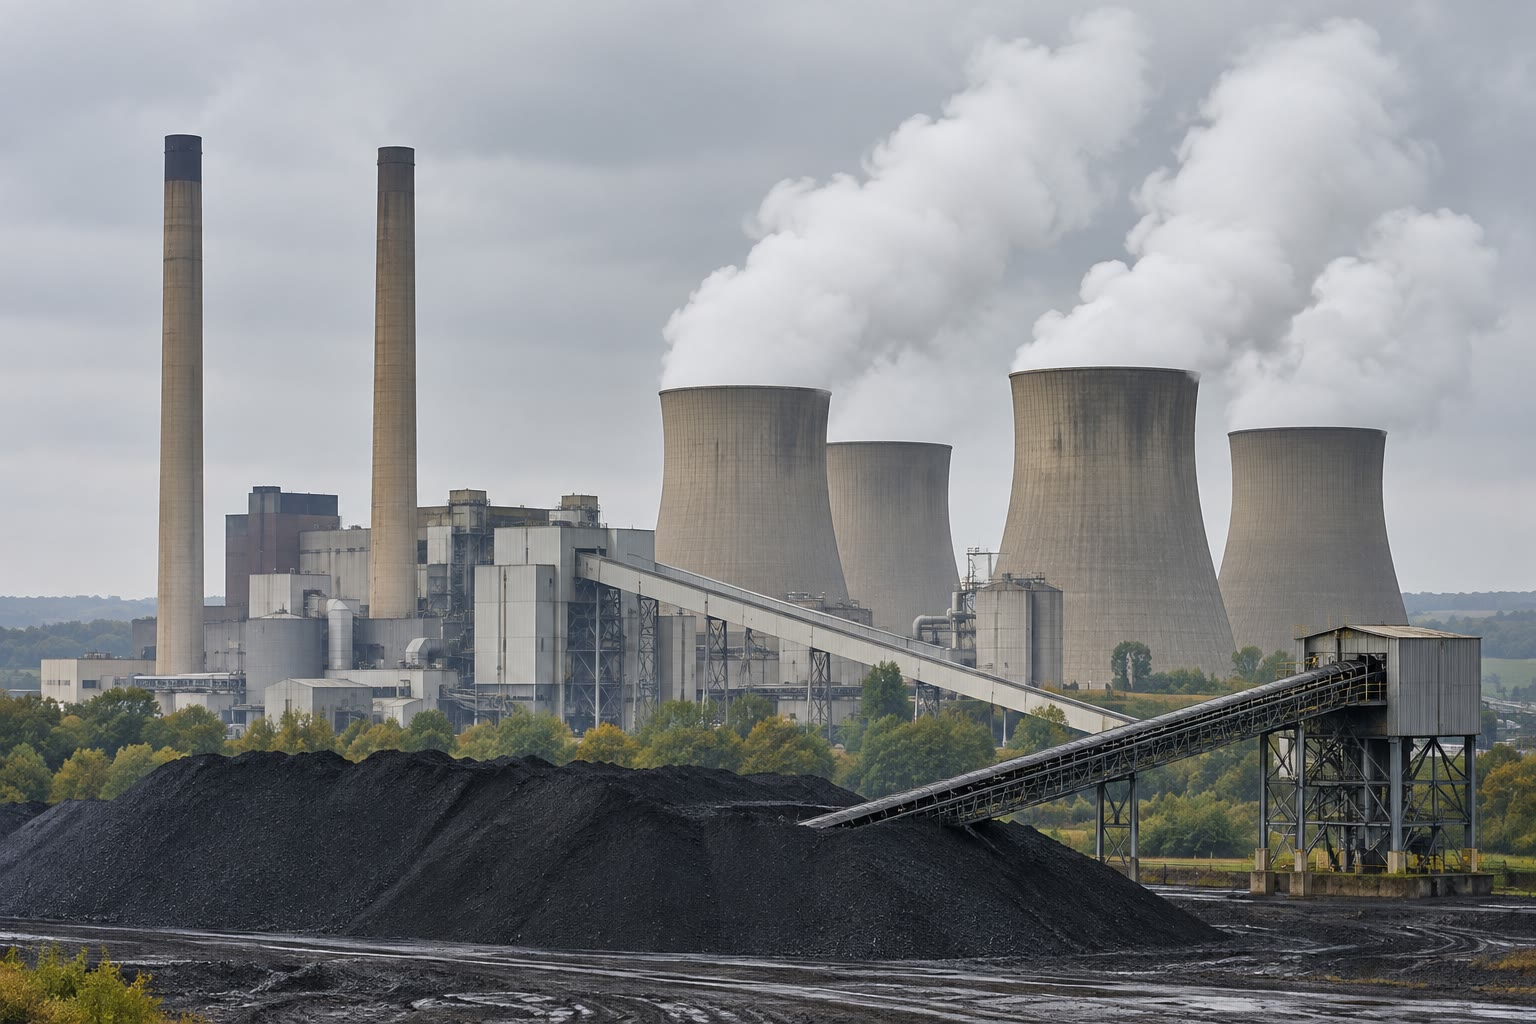
\includegraphics[width=\linewidth,height=4.6cm,keepaspectratio]{images/book1/ai/g8-coal-plant.jpg}

{\small Pembangkit listrik tenaga batu bara.}
\end{minipage}\hfill
\begin{minipage}[t]{0.48\linewidth}\centering
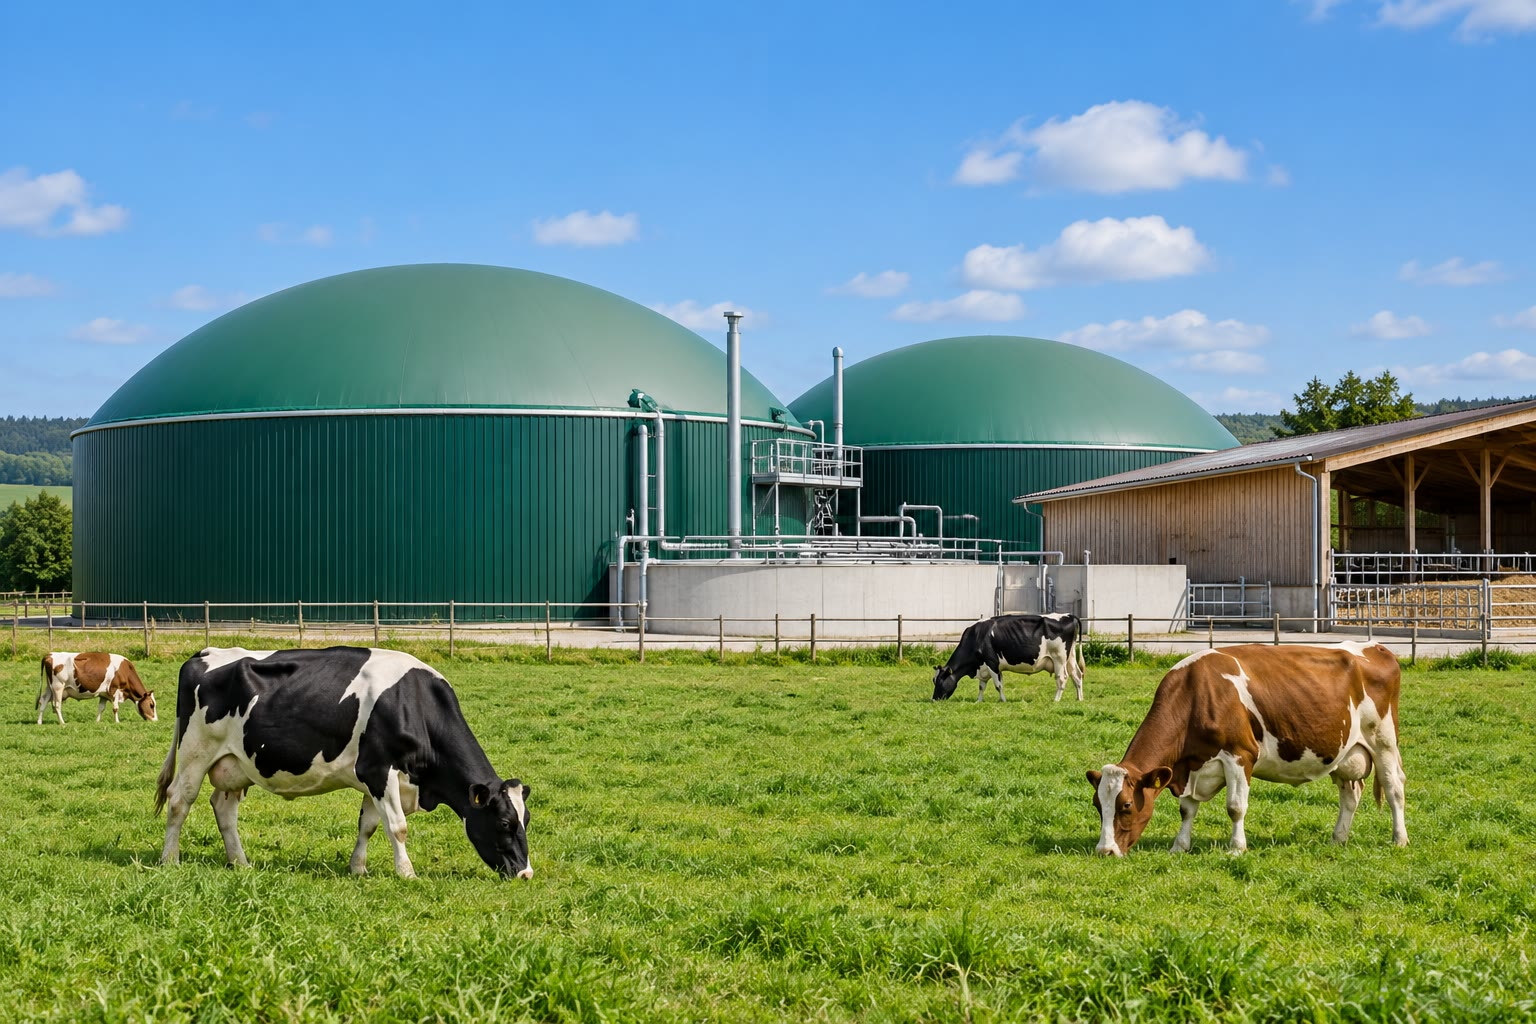
\includegraphics[width=\linewidth,height=4.6cm,keepaspectratio]{images/book1/ai/g8-biogas-farm.jpg}

{\small Instalasi biogas di sebuah peternakan: kotoran ternak menjadi
\omterm{def:g8:combustion-and-fuels:fossil}{bahan bakar terbarukan}.}
\end{minipage}
\end{omfigure}

\section{Latihan}

\begin{exercise}[$\star$]\label{exo:g8:combustion-and-fuels:1}
Tuliskan \omterm{def:g8:balanced-equations:equation}{persamaan setara} \omterm{def:g8:combustion-and-fuels:complete}{pembakaran sempurna} karbon.
\end{exercise}

\begin{exercise}[$\star$]\label{exo:g8:combustion-and-fuels:2}
Apa perbedaan antara \omterm{def:g8:combustion-and-fuels:complete}{pembakaran sempurna} dan \omterm{def:g8:combustion-and-fuels:complete}{pembakaran tidak sempurna}?
\end{exercise}

\begin{exercise}[$\star$]\label{exo:g8:combustion-and-fuels:3}
Mengapa karbon monoksida disebut bahaya yang senyap?
\end{exercise}

\begin{exercise}[$\star$]\label{exo:g8:combustion-and-fuels:4}
Fosil atau terbarukan: batu bara, kayu, gas alam, biogas, bensin, etanol
dari bit gula?
\end{exercise}

\begin{exercise}[$\star\star$]\label{exo:g8:combustion-and-fuels:5}
Tuliskan \omterm{def:g8:balanced-equations:equation}{persamaan setara} \omterm{def:g8:combustion-and-fuels:complete}{pembakaran sempurna} propana, \ce{C3H8}.
\end{exercise}

\begin{exercise}[$\star\star$]\label{exo:g8:combustion-and-fuels:6}
Etanol, \ce{C2H6O}, \omterm{def:g4:what-a-fire-needs:burning}{terbakar} sempurna dalam oksigen. Setarakan
\ce{C2H6O + O2 -> CO2 + H2O}. % ce-unbalanced-ok (to balance)
\end{exercise}

\begin{exercise}[$\star\star$]\label{exo:g8:combustion-and-fuels:7}
Panci yang dipegang di atas nyala kuning menjadi hitam di bagian
bawahnya. Zat hitam apakah itu? Apa yang ditunjukkannya tentang
\omterm{def:g4:what-a-fire-needs:burning}{pembakaran} itu?
\end{exercise}

\begin{exercise}[$\star\star$]\label{exo:g8:combustion-and-fuels:8}
Bacalah kurva karbon dioksida: kira-kira berapa banyak karbon dioksida
di \omterm{def:g4:air-a-mixture-of-gases:air}{udara} pada tahun 1980 dan pada tahun 2000? Berapa ppm kenaikannya
dalam dua puluh tahun itu?
\end{exercise}

\begin{exercise}[$\star\star$]\label{exo:g8:combustion-and-fuels:9}
Mengapa membakar kayu, dari tahun ke tahun, menambah lebih sedikit
karbon dioksida ke \omterm{def:g4:air-a-mixture-of-gases:air}{udara} daripada membakar batu bara, padahal keduanya
menghasilkan karbon dioksida?
\end{exercise}

\begin{exercise}[$\star\star$]\label{exo:g8:combustion-and-fuels:10}
Setarakan \omterm{def:g8:combustion-and-fuels:complete}{pembakaran tidak sempurna} karbon menjadi karbon monoksida,
\ce{C + O2 -> CO}. % ce-unbalanced-ok (to balance)
\end{exercise}

\begin{exercise}[$\star\star\star$]\label{exo:g8:combustion-and-fuels:11}
Dari tahun 1959 (316 ppm) sampai 2025 (427 ppm), berapa persen kenaikan
karbon dioksida di \omterm{def:g4:air-a-mixture-of-gases:air}{udara}? Bulatkan ke bilangan bulat terdekat.
\end{exercise}

\begin{exercise}[$\star\star\star$]\label{exo:g8:combustion-and-fuels:12}
Sebuah pemanas gas dipakai di ruangan kecil dengan jendela tertutup.
Jelaskan, dengan dua persamaan dari bab ini, bagaimana \omterm{def:g4:what-a-fire-needs:burning}{pembakaran} itu
dapat berubah dari sempurna menjadi tidak sempurna seiring berjalannya
waktu, dan mengapa hal itu berbahaya.
\end{exercise}

\section{Soal: Kompor di Dalam Tenda}

\begin{problem}[{Soal akhir pekan --- kompor kemah, gas yang dibakarnya,
apa yang dihasilkannya, dan mengapa kompor itu tidak pernah boleh
masuk tenda}]
\label{pb:g8:combustion-and-fuels:1}
% ledger: ghs:propane
Sebuah kompor kemah membakar propana, \ce{C3H8}, dari tabung kecil yang
berisi \qty{450}{g} propana. Di \omterm{def:g4:air-a-mixture-of-gases:air}{udara} terbuka nyalanya biru. Pakailah
perbandingan massa berikut, yang dihitung dari \omterm{def:g8:balanced-equations:equation}{persamaan setara}:
\qty{44}{g} propana yang \omterm{def:g4:what-a-fire-needs:burning}{terbakar} sempurna menghasilkan \qty{132}{g}
karbon dioksida.

\medskip
\noindent\textbf{Bagian I --- Persamaan-persamaannya.}
\begin{enumerate}
  \item Tuliskan \omterm{def:g8:balanced-equations:equation}{persamaan setara} \omterm{def:g8:combustion-and-fuels:complete}{pembakaran sempurna} propana.
  \item Periksalah dengan menghitung \omterm{def:g7:atoms-and-molecules:atom}{atom} setiap jenis di setiap ruas.
  \item Setarakan \omterm{def:g8:combustion-and-fuels:complete}{pembakaran tidak sempurna}
        \ce{C3H8 + O2 -> CO + H2O}. % ce-unbalanced-ok (to balance)
  \item Manakah di antara keduanya yang memerlukan lebih banyak oksigen
        per \omterm{def:g7:atoms-and-molecules:molecule}{molekul} propana?
\end{enumerate}

\medskip
\noindent\textbf{Bagian II --- Di dalam tenda.}
\begin{enumerate}[resume]
  \item Kompor yang dinyalakan di dalam tenda tertutup segera menyala
        dengan nyala kuning. Jelaskan mengapa.
  \item Gas berbahaya apa yang kemudian terbentuk? Sebutkan dua sifatnya
        yang membuatnya sulit disadari.
  \item Tabung propana memuat dua piktogram. Sebutkan keduanya dan
        jelaskan arti masing-masing.
  \item Berikan dua aturan untuk memakai kompor kemah dengan aman.
\end{enumerate}

\medskip
\noindent\textbf{Bagian III --- Karbon dioksida dari satu tabung.}
\begin{enumerate}[resume]
  \item Berapa kali lebih berat karbon dioksida yang terbentuk
        dibandingkan propana yang \omterm{def:g4:what-a-fire-needs:burning}{terbakar}?
  \item Dari mana gram-gram tambahan itu berasal?
  \item Apakah propana \omterm{def:g8:combustion-and-fuels:fossil}{bahan bakar fosil} atau \omterm{def:g8:combustion-and-fuels:fossil}{bahan bakar terbarukan}?
        Apakah membakarnya menambah karbon dioksida di \omterm{def:g4:air-a-mixture-of-gases:air}{udara}?
  \item Hitung massa karbon dioksida yang dilepaskan ketika satu tabung
        \qty{450}{g} \omterm{def:g4:what-a-fire-needs:burning}{terbakar} sempurna seluruhnya.
\end{enumerate}
\end{problem}
